\chapter{Experiments}
The main purpose of this chapter of this paper is to compare animations
generated procedurally with the use of Ik with baked animations. The comparison
is broken up into two categories - visual and performance. 

\section{Baked animations}
 In order to conduct the experiments comprised of visual and performance
 comparisons, a second set of animations were created each of the examples which
 are shown in the demo application. Below is an explanation of the process of
 creating this second set of animations.

\subsubsection{Spider}
The baked animation version of the spider was animated in Blender. The set
consists of idle and walking animations which, in Blender, are placed on
a single timeline, one after the other (Figure \ref{fig:timeline}). Once the model is imported
into Unity, the animations can be broken up into their separate cases, as shown
earlier in the "tools" chapter of this paper (Figure \ref{fig:anim_chunk}). 

\begin{figure}[h!]
    \centering
    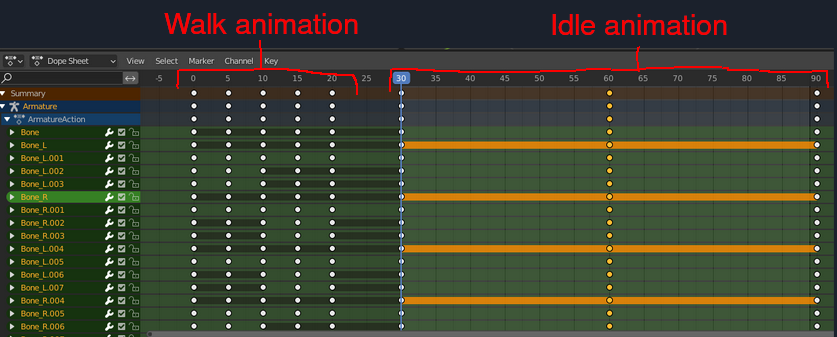
\includegraphics[width=0.7\textwidth]{grafika/blender_timeline.png}
    \caption{Two animations on a single timeline}
    \label{fig:timeline}
\end{figure}

Once the animations have been imported, a new animation controller is created
for the new spider. The animations are added, this time with the use of a blend
tree (Figure \ref{fig:s_blendtree}) to, as the name suggests, blend between the
animation smoothly CITE. A third animation state is added to the blend tree
which is the equivalent of the walking animation, but the animation speed is set
to a negative value. This plays the animation in reverse and is used when the
spider is walking backwards. 

\begin{figure}[h!]
    \centering
    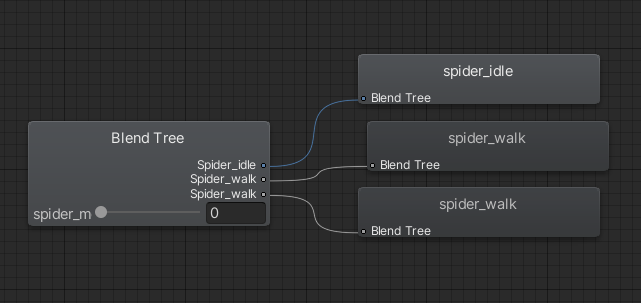
\includegraphics[width=0.7\textwidth]{grafika/spider_blend.png}
    \caption{Blend tree containing animations for the spider}
    \label{fig:s_blendtree}
\end{figure}

A variable named \textit{spider\_movement} is created in order to control the
animations that are to be played in a given situation, and the manner in which
the transitions should be blended. The thresholds for each animation can be
defined in the blend tree's configuration in the animator (Figure ref).

\begin{figure}[h!]
    \centering
    \captionsetup{justification=centering}
    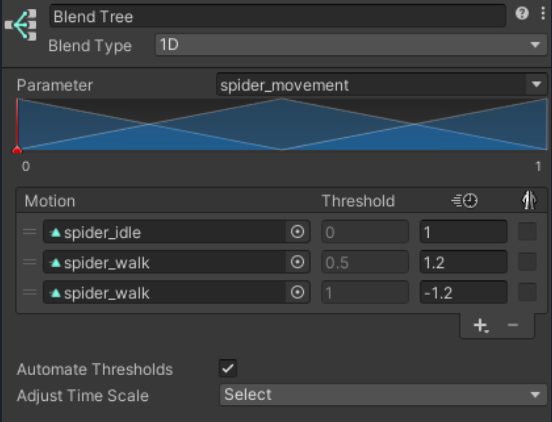
\includegraphics[width=0.7\textwidth]{grafika/spider_blendconf.png}
    \caption{Configuration of the spider's blend tree which is dependent on
    the \textit{spider\_movement} variable}
    \label{fig:s_blendconf}
\end{figure}

In the spiders movement script, this variable can then be set in reaction to
certain inputs so that the proper animation is activated each given situation.
To achieve the transition blending, the \textit{spider\_movement} variable
should not be set outright to the value which corresponds to the next animation
state. Instead, the \textit{\_animator.SetFloat} method is used, where the
\textit{\_animator} is a reference to the spider's Animator component. This
method allows the value of spider\_movement to be interpolated from the value of
the current animation state to another desired value.
\newline
\begin{lstlisting}[basicstyle=\footnotesize, numbers=none,frame=single,
caption={Transitioning to the spider's idle animation using the
\textit{SetFloat} method},captionpos=b, label=stretch, language={[Sharp]c}]
    if (verticalAxis == 0f && horizontalAxis == 0f)
        _animator.SetFloat("spider_movement", 0f, 0.05f, Time.deltaTime);
\end{lstlisting}

This version of the spider has its movement based on the spider from the game
Minecraft, which means that its rotation on the x and z axes is locked. The
spider can rotate about the y-axis when turning to face a different direction,
but it will not adjust to variations in the surface which it walks upon.
Additionally, when the spider encounters a vertical wall, it begins moving
vertically instead of horizontally until it scales the entire obstacle.

\subsubsection{Human}
The baked version of the human character, which performs an animation sequence
consisting of pressing buttons, is also animated in Blender. The animation plays
one full sequence of pressing a single button. Chunks of the same animation are
used in the IK version of this animation sequence which is described in the
previous chapter, however the baked animation utilizes the full animation while
the IK version uses only the beginning and the end. Nevertheless, the animation
is still broken up into three parts when imported into Unity: the raising of the
hand, the button pressing motion, and the lowering of the hand (Figure
\ref{fig:bp_clips}). This is done because when the character is pressing
multiple buttons in a row, the hand should not be lowered to its starting
position after every press.

\begin{figure}[h!]
    \centering
    \captionsetup{justification=centering}
    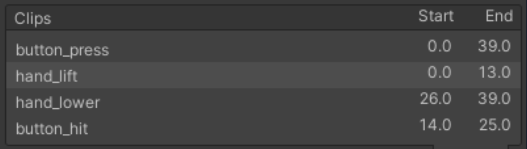
\includegraphics[width=0.7\textwidth]{grafika/bp_clips.png}
    \caption{The full button press animation is broken up into 3 separate clips}
    \label{fig:bp_clips}
\end{figure}

Another animation controller is created for this version of the human. Unlike
the spider example, the animation states do not have to be blended as they are
all clips which combine to create the full button press animation, and the
transitions are seamless as they are. Because of this, the animation states for
the three animation clips are not part of a blend tree, and instead are just
"floating" states with no defined transitions. The logic for which animation
should be played at what time is defined in the main script attached to the
character. 

The script is a simplified version of the one which controls the IK version of
this character's animation. It has no need for the public parameters present in
it's IK version because there is no IK rig, IK target, or button transforms
which it needs to control. Due to this, there is no list containing the sequence
of buttons to be pressed. It is instead replaced by an integer value which
dictates the number of button presses to execute in one animation sequence in
order to convey the idea that the character is pressing multiple buttons in
a sequence. 

As with the IK version of this script, the logic is based on a set of coroutines
which control the flow of the animation sequence. However, only the
\textit{HandAnimation} coroutine is used as a building block for the sequence
because the whole action is now constructed using baked animations. When the
script receives an input and the animation is not already playing, the sequence
begins by setting the \textit{idle} variable to true to prevent the sequence
from being repeated while it is still in progress. All required animation clips
are then set off one after the other, starting with the animation to lift the
hand. This is then followed by the animation clip which is responsible for
hitting the button, and it is repeated in a loop for a number of times defined
by the button press count parameter. Finally, the animation clip for lowering
the hand is executed, and the \textit{idle} boolean is set to false before
terminating the sequence.

\section{Visual Comparison}

\subsubsection{Spider}
\subsubsection{Human}

\section{Performance Comparison}

\subsubsection{Spider}
\subsubsection{Human}
